\tnote{Fritz}{The code should be a direct mapping of the application design onto the architecture and technologies as specified by the architecture design. As such the code should be largely self-documenting. However, if there are any tricky aspects around the implementation mapping which you would like to document outside the code, it can be done in this section.}

\tnote{Vreda}{I have drawn the following diagram to show the components of how I see the ideal memo. This is of course open for discussion and changes. I  also did not know where this idea will fit in the final design and documentation so I just put it here. I still have to learn how to integrate a Magic Draw project integrate in the documentation.}

\begin{figure}[ht]
\caption{Components of a memo specification}
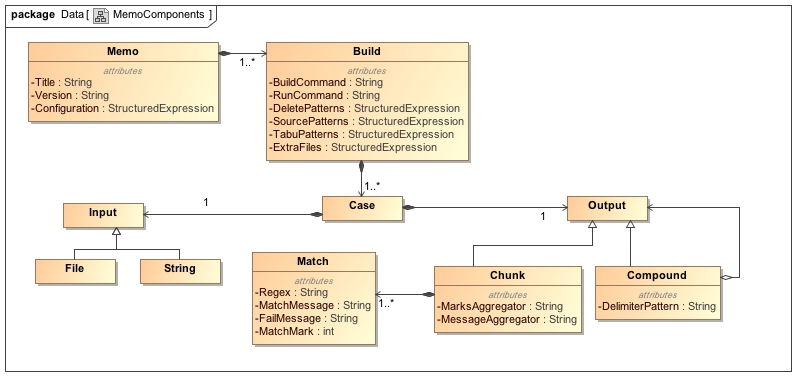
\includegraphics[width=16cm]{MemoComponents.jpg}
\end{figure}
